\chapter{Amélioration technique de KOOPT}
\label{sec:Amélioration technique de KOOPT}

\section*{Introduction}


Ce Chapitre présente les missions qui me sont confiées au niveau de l’amélioration technique de KOOPT et qui consiste l'évolution de certains IHM de l’application ainsi que le développement des sous-fonctionnalités de KOOPT.
\addcontentsline{toc}{section}{Introduction.}


\section{L’utilisation de KOOPT}

\subsection{Les écrans d’aide KOOPT}
Afin de faciliter l’utilisation de KOOPT pour les utilisateurs et de les guider sur le fonctionnement général de KOOPT, on a mis en place des écrans d’aide pour toute l’application, accessibles dans toutes les IHM de KOOPT.
Pour cela, on a utilisé la librairie ShowCaseView.

\subsection{ShowCaseView}
La bibliothèque ShowcaseView (SCV) est conçue pour mettre en évidence des parties spécifiques d'applications à l'utilisateur avec une superposition distinctive et attrayante. Cette bibliothèque est idéale pour indiquer les points d'intérêt pour les utilisateurs, les gestes ou les objets obscurs mais utiles.

 \begin{figure}[H]
\begin{center}
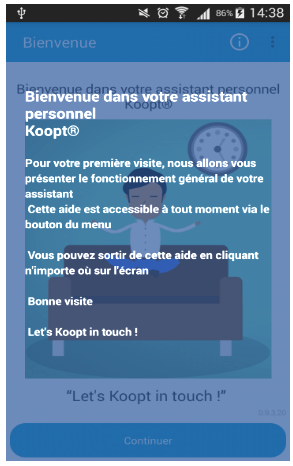
\includegraphics[width=0.5\linewidth]{images/help}
\end{center}
\caption{Écran d'aide de la page d'accueil KOOPT}
\label{fig:12}
\end{figure}
Target: 
 
ShowCaseView fournit la possibilité d’utiliser des targets,  qui sont sous forme de cercles, qui 
mettent  le focus sur un objet spécifique dans un IHM afin de pouvoir aider et guider l’utilisateur sur l’utilisation de cet objet. 

 \begin{figure}[H]
\begin{center}
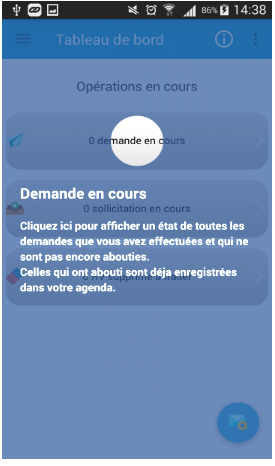
\includegraphics[width=0.5\linewidth]{images/helptarget}
\end{center}
\caption{Écran d'aide du Tableau de bord KOOPT}
\label{fig:13}
\end{figure}

\subsection{Inconvénient}

ShowCaseView offre un support et une aide pour l’utilisateur de l’application à travers la manipulation facile et flexible des Targets.
Le positionnement d'un texte spécifique à une Target est ingérable et produit un écran d’aide mal structuré dans certains cas où l’application est lancée sur des smartphones avec un petit écran.

\section{Alerte des Koopters}
Après une organisation de rendez-vous effectuée par un utilisateur de KOOPT avec d’autres Koopters,  l’application donne la possibilité d’alerter ces derniers s'il n’y a aucune réponse reçue  de leur part. pour cela on a mis en place un système d’envoi de SMS qui permettra aux organisateurs de rendez-vous d’envoyer un SMS d’une façon automatique aux autres Koopters concernés dont l’application KOOPT est désactivée afin de pouvoir la relancer.

 \begin{figure}[H]
\begin{center}
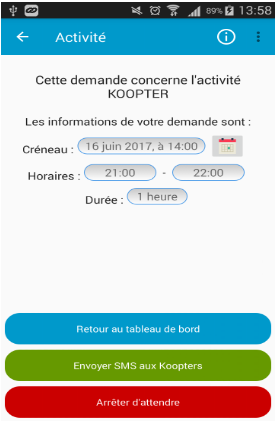
\includegraphics[width=0.5\linewidth]{images/sendsms}
\end{center}
\caption{IHM KOOPT qui permet l'envoi de SMS à un Koopter}
\label{fig:15}
\end{figure}

Pour cela on a utilisé API SMSManager.

\subsection{SMSManager}
SmsManager est la classe qui  gère l’envoi des  SMS dans une application Android . Il n'est pas possible d'avoir une instance de cette classe, mais il faudra utiliser une méthode statique SmsManager.getDefault() pour en récupérer une par défaut.

SmsManager sms = SmsManager.getDefault();

Sécurité : 
Pour envoyer un SMS, il faut d'abord autoriser l'application et ajouter la permission d’envoi des SMS Dans le fichier AndroidManifest.xml de l’application :
<uses-permission android:name="android.permission.SEND\_SMS"/>
\subsection{Contraintes}
Les SMS ont une taille de 160 caractères maximum. Au delà, il sera nécessaire de découper le texte en bloc de 160 caractères et de les envoyer les uns après les autres.
Dans KOOPT on a choisi un message réduit qui ne dépasse pas 160 caractères et qui contient toutes les informations nécessaires pour alerter les Koopters.

\section{Contact pour nouvelle activité}

KOOPT donne la possibilité à ses utilisateurs de suggérer de nouvelles activités mais pas d’une façon automatique pour des raisons de control de l’application. pour cela, on a implémenté un mécanisme de contact avec l’administrateur de KOOPT par Email dans lequel l’utilisateur propose l’activité qu’il souhaiterait ajouter à la liste des activités déjà existantes KOOPT.

 \begin{figure}[H]
\begin{center}
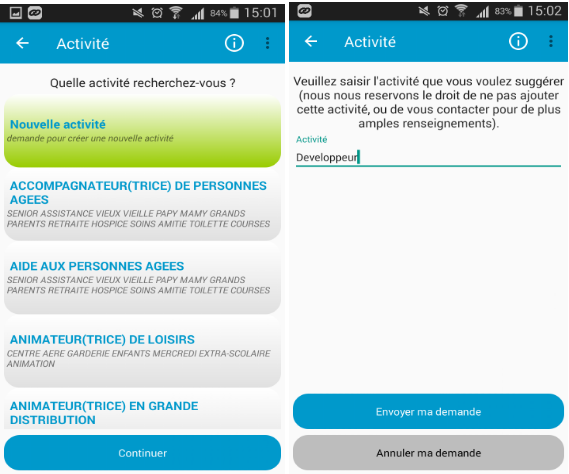
\includegraphics[width=1\linewidth]{images/newactivite}
\end{center}
\caption{Suggestion d'ajout d'une nouvelle activité à KOOPT}
\label{fig:16}
\end{figure}


 \begin{figure}[H]
\begin{center}
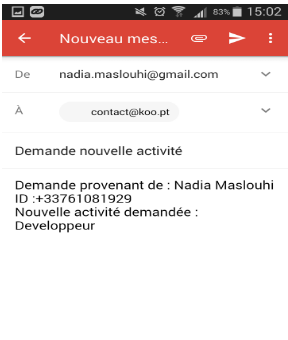
\includegraphics[width=0.5\linewidth]{images/sendmail}
\end{center}
\caption{Envoi d'Email au directeur de KOOPT}
\label{fig:17}
\end{figure}

Après la saisie de l’activité souhaitée, l’utilisateur clique sur "Envoyer la demande". L’application Email du smartphone s'ouvre avec un Email prés-rempli. l'utilisateur n'as plus qu'a cliquer sur le bouton qui renvoyait l'Email.
L'administrateur KOOPT traite les demandes reçues, et ajoute les activités par une application dédiée. 
\subsection{Inconvenient}
L’envoi d’un Email automatique reste toujours un obstacle pour KOOPT et aussi pour d’autres applications car la programmation et la configuration d’un tel mécanisme nécessite la récupération des identifiants qui sont propre à l’utilisateur (Email et mot de passe) pour pouvoir s’authentifier et envoyer un Email directement sans passer par des applications intermédiaires d'Email.

Pour cela dans KOOPT on était censé de donner le choix à l’utilisateur pour sélectionner l’application avec laquelle il veut envoyer son Email (Exemple : Gmail).


\section{Gestion des notifications }
KOOPT s’appuie beaucoup sur les notifications lors de son utilisation.
en lançant KOOPT une notification KOOPT apparaît sur le smartphone et qui reste persistante sauf si l’utilisateur a quitté KOOPT, En cliquant sur cette dernière, l’application se lancera de nouveau.

KOOPT utilise aussi les notifications pour alerter l’utilisateur dans plusieurs cas (Réception d’une sollicitation , Réception d’une confirmation de rendez-vous …). 
Toutes ces notifications nécessitent une gestion pour éviter les notifications obsolètes, c’est à dire le cas où l’utilisateur a toujours une notification pour ouvrir un IHM spécifique qu’il a déjà ouvert. 

Donc on a implémenté un mécanisme qui teste à chaque apparition d’une notification si l’IHM demandée a déjà été ouverte par l’utilisateur. dans ce cas la notification sera supprimée automatiquement en utilisant le NotificationManager.
\subsection{Notification Manager}
Pour envoyer des notifications, il faut passer par  l'instance du service de notifications d'Android (Notification Manager). Il s'agit d'un service gérant pour toutes les applications ces notifications. Celui-ci va trier ces notifications par ordre de priorité (qui correspond au paramètre notification when précisant quand la notification a été envoyée) pour en informer ensuite l'utilisateur.\cite{notification}
 
Notification Manager permet d’envoyer, modifier et annuler une notification grâce a son identifiant.

\section{Les Settings KOOPT  }

Dans KOOPT, il est nécessaire de garder en mémoire les différentes informations d’un utilisateur (Numéro de téléphone , Code d'accès, nom, adresse, activités …) même suite à une fermeture de l’application. La solution est de créer des Settings (Instance de  SharedPreferences) pour stocker toutes les informations nécessaires afin qu’il puisse les modifier ultérieurement.


\subsection{Changement du Code d’accès KOOPT}

Le code d’accès fait parti des informations qui sont stockées dans les settings de KOOPT et que l’utilisateur a le droit de modifier.
La modification du code d’accès se fait à l’aide du web Service KOOPT\_changePassword qui a pour rôle le changement du mot de passe d’un utilisateur en passant par plusieurs étapes : 

- La vérification de l’ancien code d'accès.

- La génération d’un code de confirmation à 6 chiffres qui sera envoyé à l’utilisateur par un SMS ( Valable 10 minutes).

- La vérification du code de confirmation et du délai de confirmation
 
Le web Service a été développé à travers la plateforme Talend (Talend Open Studio) par des composants dédiés aux fonctionnalités ESB.
 
 \begin{figure}[H]
\begin{center}
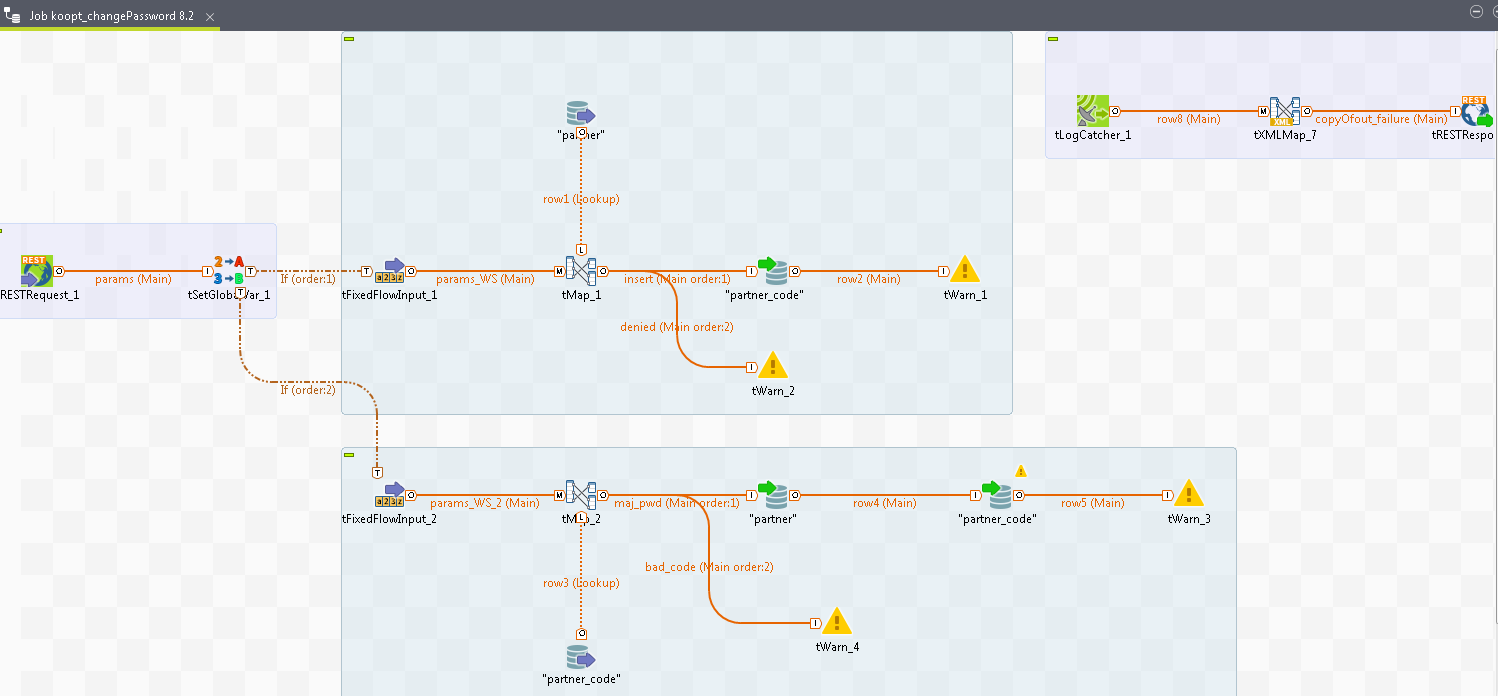
\includegraphics[width=1\linewidth]{images/webservice}
\end{center}
\caption{Web service ChangePassword\_KOOPT}
\label{fig:18}
\end{figure}
 
Le web service renvoie des réponses qui contiennent soit des objets ( code de confirmation généré) ou des messages pour montrer le résultat des vérifications réalisées. 
Suite à ses réponses, on gère la modification du code d'accès, préalablement cryptée, en le modifiant dans les Settings KOOPT.


